
% % bare_jrnl_compsoc.tex % V1.4b % 2015/08/26 % by Michael Shell % See:
% % http://www.michaelshell.org/ % for current contact information.
% % % This is a skeleton file demonstrating the use of IEEEtran.cls % (requires
% IEEEtran.cls version 1.8b or later) with an IEEE % Computer Society journal
% paper.
% % % Support sites:
% % http://www.michaelshell.org/tex/ieeetran/ % http://www.ctan.org/pkg/ieeetran
% % and % http://www.ieee.org/

% %************************************************************************* %
% Legal Notice:
% % This code is offered as-is without any warranty either expressed or %
% implied; without even the implied warranty of MERCHANTABILITY or % FITNESS FOR
% A PARTICULAR PURPOSE! % User assumes all risk.
% % In no event shall the IEEE or any contributor to this code be liable for %
% any damages or losses, including, but not limited to, incidental, %
% consequential, or any other damages, resulting from the use or misuse % of any
% information contained here.
% % % All comments are the opinions of their respective authors and are not %
% necessarily endorsed by the IEEE.
% % % This work is distributed under the LaTeX Project Public License (LPPL) % (
% http://www.latex-project.org/ ) version 1.3, and may be freely used, %
% distributed and modified. A copy of the LPPL, version 1.3, is included % in
% the base LaTeX documentation of all distributions of LaTeX released %
% 2003/12/01 or later.
% % Retain all contribution notices and credits.
% % ** Modified files should be clearly indicated as such, including  ** % **
% renaming them and changing author support contact information. **
% %*************************************************************************


% *** Authors should verify (and, if needed, correct) their LaTeX system  ***
% *** with the testflow diagnostic prior to trusting their LaTeX platform ***
% *** with production work. The IEEE's font choices and paper sizes can   ***
% *** trigger bugs that do not appear when using other class files.       ***   
%                       *** The testflow support page is at:
% http://www.michaelshell.org/tex/testflow/


\documentclass[10pt,journal,compsoc]{IEEEtran}
%  If IEEEtran.cls has not been installed into the LaTeX system files, manually
% specify the path to it like:
% \documentclass[10pt,journal,compsoc]{../sty/IEEEtran}





% Some very useful LaTeX packages include:
% (uncomment the ones you want to load)


% *** MISC UTILITY PACKAGES ***  \usepackage{ifpdf} Heiko Oberdiek's ifpdf.sty
% is very useful if you need conditional compilation based on whether the output
% is pdf or dvi.
% usage:
% \ifpdf % pdf code \else % dvi code \fi The latest version of ifpdf.sty can be
% obtained from:
% http://www.ctan.org/pkg/ifpdf Also, note that IEEEtran.cls V1.7 and later
% provides a builtin \ifCLASSINFOpdf conditional that works the same way.
% When switching from latex to pdflatex and vice-versa, the compiler may have to
% be run twice to clear warning/error messages.






% *** CITATION PACKAGES ***
\ifCLASSOPTIONcompsoc
  % IEEE Computer Society needs nocompress option requires cite.sty v4.0 or
  % later (November 2003)
  \usepackage[nocompress]{cite}
\else
  % normal IEEE
  \usepackage{cite}
\fi
% cite.sty was written by Donald Arseneau V1.6 and later of IEEEtran pre-defines
% the format of the cite.sty package \cite{} output to follow that of the IEEE.
% Loading the cite package will result in citation numbers being automatically
% sorted and properly "compressed/ranged". e.g., [1], [9], [2], [7], [5], [6]
% without using cite.sty will become [1], [2], [5]--[7], [9] using cite.sty.
% cite.sty's \cite will automatically add leading space, if needed. Use
% cite.sty's noadjust option (cite.sty V3.8 and later) if you want to turn this
% off such as if a citation ever needs to be enclosed in parenthesis.
% cite.sty is already installed on most LaTeX systems. Be sure and use version
% 5.0 (2009-03-20) and later if using hyperref.sty.
% The latest version can be obtained at:
% http://www.ctan.org/pkg/cite The documentation is contained in the cite.sty
% file itself.
%  Note that some packages require special options to format as the Computer
% Society requires. In particular, Computer Society  papers do not use
% compressed citation ranges as is done in typical IEEE papers (e.g., [1]-[4]).
% Instead, they list every citation separately in order (e.g., [1], [2], [3],
% [4]). To get the latter we need to load the cite package with the nocompress
% option which is supported by cite.sty v4.0 and later. Note also the use of a
% CLASSOPTION conditional provided by IEEEtran.cls V1.7 and later.





% *** GRAPHICS RELATED PACKAGES ***
\ifCLASSINFOpdf
  \usepackage[pdftex]{graphicx}
  \usepackage{csvsimple}
\usepackage{array}
\usepackage{float}
\usepackage{amsmath}
\usepackage{pgfplotstable}
  % declare the path(s) where your graphic files are
  % \graphicspath{{../pdf/}{../jpeg/}} and their extensions so you won't have to
  % specify these with every instance of \includegraphics
  % \DeclareGraphicsExtensions{.pdf,.jpeg,.png}
\else
  % or other class option (dvipsone, dvipdf, if not using dvips). graphicx will
  % default to the driver specified in the system graphics.cfg if no driver is
  % specified.
  % \usepackage[dvips]{graphicx} declare the path(s) where your graphic files
  % are \graphicspath{{../eps/}} and their extensions so you won't have to
  % specify these with every instance of \includegraphics
  % \DeclareGraphicsExtensions{.eps}
\fi
% graphicx was written by David Carlisle and Sebastian Rahtz. It is required if
% you want graphics, photos, etc. graphicx.sty is already installed on most
% LaTeX systems. The latest version and documentation can be obtained at:
% http://www.ctan.org/pkg/graphicx Another good source of documentation is
% "Using Imported Graphics in LaTeX2e" by Keith Reckdahl which can be found at:
% http://www.ctan.org/pkg/epslatex  latex, and pdflatex in dvi mode, support
% graphics in encapsulated postscript (.eps) format. pdflatex in pdf mode
% supports graphics in .pdf, .jpeg, .png and .mps (metapost) formats. Users
% should ensure that all non-photo figures use a vector format (.eps, .pdf,
% .mps) and not a bitmapped formats (.jpeg, .png). The IEEE frowns on bitmapped
% formats which can result in "jaggedy"/blurry rendering of lines and letters as
% well as large increases in file sizes.
%  You can find documentation about the pdfTeX application at:
% http://www.tug.org/applications/pdftex






% *** MATH PACKAGES ***  \usepackage{amsmath} A popular package from the
% American Mathematical Society that provides many useful and powerful commands
% for dealing with mathematics.
%  Note that the amsmath package sets \interdisplaylinepenalty to 10000 thus
% preventing page breaks from occurring within multiline equations. Use:
% \interdisplaylinepenalty=2500 after loading amsmath to restore such page
% breaks as IEEEtran.cls normally does. amsmath.sty is already installed on most
% LaTeX systems. The latest version and documentation can be obtained at:
% http://www.ctan.org/pkg/amsmath





% *** SPECIALIZED LIST PACKAGES ***  \usepackage{algorithmic} algorithmic.sty
% was written by Peter Williams and Rogerio Brito.
% This package provides an algorithmic environment fo describing algorithms.
% You can use the algorithmic environment in-text or within a figure environment
% to provide for a floating algorithm. Do NOT use the algorithm floating
% environment provided by algorithm.sty (by the same authors) or algorithm2e.sty
% (by Christophe Fiorio) as the IEEE does not use dedicated algorithm float
% types and packages that provide these will not provide correct IEEE style
% captions. The latest version and documentation of algorithmic.sty can be
% obtained at:
% http://www.ctan.org/pkg/algorithms Also of interest may be the (relatively
% newer and more customizable) algorithmicx.sty package by Szasz Janos:
% http://www.ctan.org/pkg/algorithmicx




% *** ALIGNMENT PACKAGES ***  \usepackage{array} Frank Mittelbach's and David
% Carlisle's array.sty patches and improves the standard LaTeX2e array and
% tabular environments to provide better appearance and additional user
% controls. As the default LaTeX2e table generation code is lacking to the point
% of almost being broken with respect to the quality of the end results, all
% users are strongly advised to use an enhanced (at the very least that provided
% by array.sty) set of table tools. array.sty is already installed on most
% systems. The latest version and documentation can be obtained at:
% http://www.ctan.org/pkg/array


% IEEEtran contains the IEEEeqnarray family of commands that can be used to
% generate multiline equations as well as matrices, tables, etc., of high
% quality.




% *** SUBFIGURE PACKAGES *** \ifCLASSOPTIONcompsoc
% \usepackage[caption=false,font=footnotesize,labelfont=sf,textfont=sf]{subfig}
% \else \usepackage[caption=false,font=footnotesize]{subfig} \fi subfig.sty,
% written by Steven Douglas Cochran, is the modern replacement for
% subfigure.sty, the latter of which is no longer maintained and is incompatible
% with some LaTeX packages including fixltx2e. However, subfig.sty requires and
% automatically loads Axel Sommerfeldt's caption.sty which will override
% IEEEtran.cls' handling of captions and this will result in non-IEEE style
% figure/table captions. To prevent this problem, be sure and invoke
% subfig.sty's "caption=false" package option (available since subfig.sty
% version 1.3, 2005/06/28) as this is will preserve IEEEtran.cls handling of
% captions.
% Note that the Computer Society format requires a sans serif font rather than
% the serif font used in traditional IEEE formatting and thus the need to invoke
% different subfig.sty package options depending on whether compsoc mode has
% been enabled.
%  The latest version and documentation of subfig.sty can be obtained at:
% http://www.ctan.org/pkg/subfig




% *** FLOAT PACKAGES ***  \usepackage{fixltx2e} fixltx2e, the successor to the
% earlier fix2col.sty, was written by Frank Mittelbach and David Carlisle. This
% package corrects a few problems in the LaTeX2e kernel, the most notable of
% which is that in current LaTeX2e releases, the ordering of single and double
% column floats is not guaranteed to be preserved. Thus, an unpatched LaTeX2e
% can allow a single column figure to be placed prior to an earlier double
% column figure.
% Be aware that LaTeX2e kernels dated 2015 and later have fixltx2e.sty's
% corrections already built into the system in which case a warning will be
% issued if an attempt is made to load fixltx2e.sty as it is no longer needed.
% The latest version and documentation can be found at:
% http://www.ctan.org/pkg/fixltx2e


% \usepackage{stfloats} stfloats.sty was written by Sigitas Tolusis. This
% package gives LaTeX2e the ability to do double column floats at the bottom of
% the page as well as the top. (e.g., "\begin{figure*}[!b]" is not normally
% possible in LaTeX2e). It also provides a command:
% \fnbelowfloat to enable the placement of footnotes below bottom floats (the
% standard LaTeX2e kernel puts them above bottom floats). This is an invasive
% package which rewrites many portions of the LaTeX2e float routines. It may not
% work with other packages that modify the LaTeX2e float routines. The latest
% version and documentation can be obtained at:
% http://www.ctan.org/pkg/stfloats Do not use the stfloats baselinefloat ability
% as the IEEE does not allow \baselineskip to stretch. Authors submitting work
% to the IEEE should note that the IEEE rarely uses double column equations and
% that authors should try to avoid such use. Do not be tempted to use the
% cuted.sty or midfloat.sty packages (also by Sigitas Tolusis) as the IEEE does
% not format its papers in such ways.
% Do not attempt to use stfloats with fixltx2e as they are incompatible.
% Instead, use Morten Hogholm'a dblfloatfix which combines the features of both
% fixltx2e and stfloats:
%  \usepackage{dblfloatfix} The latest version can be found at:
% http://www.ctan.org/pkg/dblfloatfix




% \ifCLASSOPTIONcaptionsoff \usepackage[nomarkers]{endfloat}
% \let\MYoriglatexcaption\caption
% \renewcommand{\caption}[2][\relax]{\MYoriglatexcaption[#2]{#2}} \fi
% endfloat.sty was written by James Darrell McCauley, Jeff Goldberg and Axel
% Sommerfeldt. This package may be useful when used in conjunction with
% IEEEtran.cls'  captionsoff option. Some IEEE journals/societies require that
% submissions have lists of figures/tables at the end of the paper and that
% figures/tables without any captions are placed on a page by themselves at the
% end of the document. If needed, the draftcls IEEEtran class option or
% \CLASSINPUTbaselinestretch interface can be used to increase the line spacing
% as well. Be sure and use the nomarkers option of endfloat to prevent endfloat
% from "marking" where the figures would have been placed in the text. The two
% hack lines of code above are a slight modification of that suggested by in the
% endfloat docs (section 8.4.1) to ensure that the full captions always appear
% in the list of figures/tables - even if the user used the short optional
% argument of \caption[]{}.
% IEEE papers do not typically make use of \caption[]'s optional argument, so
% this should not be an issue. A similar trick can be used to disable captions
% of packages such as subfig.sty that lack options to turn off the subcaptions:
% For subfig.sty:
% \let\MYorigsubfloat\subfloat
% \renewcommand{\subfloat}[2][\relax]{\MYorigsubfloat[]{#2}} However, the above
% trick will not work if both optional arguments of the \subfloat command are
% used. Furthermore, there needs to be a description of each subfigure
% *somewhere* and endfloat does not add subfigure captions to its list of
% figures. Thus, the best approach is to avoid the use of subfigure captions
% (many IEEE journals avoid them anyway) and instead reference/explain all the
% subfigures within the main caption.
% The latest version of endfloat.sty and its documentation can obtained at:
% http://www.ctan.org/pkg/endfloat  The IEEEtran \ifCLASSOPTIONcaptionsoff
% conditional can also be used later in the document, say, to conditionally put
% the References on a page by themselves.




% *** PDF, URL AND HYPERLINK PACKAGES ***  \usepackage{url} url.sty was written
% by Donald Arseneau. It provides better support for handling and breaking URLs.
% url.sty is already installed on most LaTeX systems. The latest version and
% documentation can be obtained at:
% http://www.ctan.org/pkg/url Basically, \url{my_url_here}.





% *** Do not adjust lengths that control margins, column widths, etc. *** *** Do
% not use packages that alter fonts (such as pslatex).         *** There should
% be no need to do such things with IEEEtran.cls V1.6 and later.
% (Unless specifically asked to do so by the journal or conference you plan to
% submit to, of course. )


% correct bad hyphenation here
\hyphenation{op-tical net-works semi-conduc-tor}

\begin{document}
%  paper title Titles are generally capitalized except for words such as a, an,
% and, as, at, but, by, for, in, nor, of, on, or, the, to and up, which are
% usually not capitalized unless they are the first or last word of the title.
% Linebreaks \\ can be used within to get better formatting as desired.
% Do not put math or special symbols in the title.
\title{Laban Movement Analysis of Movements Recorded by Kinect, Using Machine Learning}
%   author names and IEEE memberships note positions of commas and nonbreaking
% spaces ( ~ ) LaTeX will not break a structure at a ~ so this keeps an author's
% name from being broken across two lines.
% use \thanks{} to gain access to the first footnote area a separate \thanks
% must be used for each paragraph as LaTeX2e's \thanks was not built to handle
% multiple paragraphs   \IEEEcompsocitemizethanks is a special \thanks that
% produces the bulleted lists the Computer Society journals use for "first
% footnote" author affiliations. Use \IEEEcompsocthanksitem which works much
% like \item for each affiliation group. When not in compsoc mode,
% \IEEEcompsocitemizethanks becomes like \thanks and \IEEEcompsocthanksitem
% becomes a line break with idention. This facilitates dual compilation,
% although admittedly the differences in the desired content of \author between
% the different types of papers makes a one-size-fits-all approach a daunting
% prospect. For instance, compsoc journal papers have the author affiliations
% above the "Manuscript received ..."  text while in non-compsoc journals this
% is reversed. Sigh.

\author{Tal~Shafir, Ran~Bernstein, Rachelle~P.~Tsachor, Karen~Studd,
and~Assaf~Schuster,~\IEEEmembership{Member,~IEEE}% <-this % stops a
% space


\thanks{This work was supported in part by the John Nuveen Center For
International Affairs at the University of Illinois at Chicago, Nuveen
International Development Fund.}% <-this % stops a 
\thanks{ This paper combines
two previous presentations: at the seventeenth International Conference on
Affective Computing and  Intelligent Interaction, Paris, France, May 2015 and at
the second International Workshop on Movement and Computing, Simon Fraser
University, Vancouver Canada, August 2015.} % 
\thanks{T. Shafir is with The Graduate School for Creative Arts Therapies, Faculty of
Social Welfare \& Health Sciences, The University of Haifa, Israel (e-mail:
tshafir1@ univ.haifa.ac.il).}% <-this % stops a 
\thanks{R. Bernstein and Assaf Schuster are with the Department of Computer Science, Technion I.I.T, Haifa
32000, Israel (e-mail:bernstein.ran@gmail.com, assaf@cs.technion.ac.il).}% <-this % stops a 
\thanks{R. P. Tsachor is with the School of Theatre \& Music, The University of Illinois at
Chicago, Chicago, IL 60607 USA (e-mail: rtsachor@uic.edu).}% 
\thanks{K. Studd is with the School of Dance, George Mason University, VA 22030, USA, (e-mail:
krnstudd@gmail.com).}% <-this % stops a 
}

% note the % following the last \IEEEmembership and also \thanks - these prevent
% an unwanted space from occurring between the last author name and the end of
% the author line. i.e., if you had this:
%  \author{....lastname \thanks{...} \thanks{...} }
% ^------------^------------^----Do not want these spaces!  a space would be
% appended to the last name and could cause every name on that line to be
% shifted left slightly. This is one of those "LaTeX things". For instance,
% "\textbf{A} \textbf{B}" will typeset as "A B" not "AB". To get "AB" then you
% have to do: "\textbf{A}\textbf{B}" \thanks is no different in this regard, so
% shield the last } of each \thanks that ends a line with a % and do not let a
% space in before the next \thanks.
% Spaces after \IEEEmembership other than the last one are OK (and needed) as
% you are supposed to have spaces between the names. For what it is worth, this
% is a minor point as most people would not even notice if the said evil space
% somehow managed to creep in.



% The paper headers \markboth{Journal of \LaTeX\ Class Files,~Vol.~14, No.~8,
% August~2015}% {Shell \MakeLowercase{\textit{et al.}}: Bare Demo of
% IEEEtran.cls for Computer Society Journals} The only time the second header
% will appear is for the odd numbered pages after the title page when using the
% twoside option.
%  *** Note that you probably will NOT want to include the author's *** *** name
% in the headers of peer review papers.                   *** You can use
% \ifCLASSOPTIONpeerreview for conditional compilation here if you desire.



% The publisher's ID mark at the bottom of the page is less important with
% Computer Society journal papers as those publications place the marks outside
% of the main text columns and, therefore, unlike regular IEEE journals, the
% available text space is not reduced by their presence.
% If you want to put a publisher's ID mark on the page you can do it like this:
% \IEEEpubid{0000--0000/00\$00.00~\copyright~2015 IEEE} or like this to get the
% Computer Society new two part style.
% \IEEEpubid{\makebox[\columnwidth]{\hfill 0000--0000/00/\$00.00~\copyright~2015
% IEEE}% \hspace{\columnsep}\makebox[\columnwidth]{Published by the IEEE
% Computer Society\hfill}} Remember, if you use this you must call
% \IEEEpubidadjcol in the second column for its text to clear the IEEEpubid mark
% (Computer Society jorunal papers don't need this extra clearance.)



% use for special paper notices \IEEEspecialpapernotice{(Invited Paper)}



% for Computer Society papers, we must declare the abstract and index terms
% PRIOR to the title within the \IEEEtitleabstractindextext IEEEtran command as
% these need to go into the title area created by \maketitle.
% As a general rule, do not put math, special symbols or citations in the
% abstract or keywords.
\IEEEtitleabstractindextext{%
\begin{abstract}
Laban Movement Analysis (LMA) is a method for describing, interpreting and
documenting all varieties of human movement. Analyzing movements using LMA is
advantageous over kinematic description of the movement, as it captures
qualitative aspects in addition to the quantitative aspects of the movement. As
such, it has many applications and its popularity is increasing in recent years
as the preferred method for movement analysis in motor research, theater training,
and the development of interactive gaming animations and robotics. In this study
we aimed to develop an automated method for recognizing 18 different Laban motor
elements (motor characteristics) from markerless 3D movement data captured by the
ubiquitous Kinect camera.  Using machine-learning methods we have succeeded to
obtain a recall rate of 38-94\% (65\% on average) and precision rate of 29-100\%
(59\% on average) for the 18 motor elements that were tested.
\end{abstract}

% Note that keywords are not normally used for peerreview papers.
\begin{IEEEkeywords}
Laban Movement Analysis, Machine Learning, Motion Capture.
\end{IEEEkeywords}}


% make the title area
\maketitle


% To allow for easy dual compilation without having to reenter the
% abstract/keywords data, the \IEEEtitleabstractindextext text will
% not be used in maketitle, but will appear (i.e., to be "transported")
% here as \IEEEdisplaynontitleabstractindextext when the compsoc 
% or transmag modes are not selected <OR> if conference mode is selected 
% - because all conference papers position the abstract like regular
% papers do.
\IEEEdisplaynontitleabstractindextext
% \IEEEdisplaynontitleabstractindextext has no effect when using
% compsoc or transmag under a non-conference mode.



% For peer review papers, you can put extra information on the cover
% page as needed:
% \ifCLASSOPTIONpeerreview
% \begin{center} \bfseries EDICS Category: 3-BBND \end{center}
% \fi
%
% For peerreview papers, this IEEEtran command inserts a page break and
% creates the second title. It will be ignored for other modes.
\IEEEpeerreviewmaketitle



\IEEEraisesectionheading{\section{Introduction}\label{sec:introduction}}
% Computer Society journal (but not conference!) papers do something unusual
% with the very first section heading (almost always called "Introduction").
% They place it ABOVE the main text! IEEEtran.cls does not automatically do
% this for you, but you can achieve this effect with the provided
% \IEEEraisesectionheading{} command. Note the need to keep any \label that
% is to refer to the section immediately after \section in the above as
% \IEEEraisesectionheading puts \section within a raised box.




% The very first letter is a 2 line initial drop letter followed
% by the rest of the first word in caps (small caps for compsoc).
% 
% form to use if the first word consists of a single letter:
% \IEEEPARstart{A}{demo} file is ....
% 
% form to use if you need the single drop letter followed by
% normal text (unknown if ever used by the IEEE):
% \IEEEPARstart{A}{}demo file is ....
% 
% Some journals put the first two words in caps:
% \IEEEPARstart{T}{his demo} file is ....
% 
% Here we have the typical use of a "T" for an initial drop letter
% and "HIS" in caps to complete the first word.
\IEEEPARstart{I}{n} recent years there has been a surge of interest in automated analysis of
human motor behavior in the fields of robotics, computer science and animation.
Computerized recognition of movement characteristics has many potential
applications: It could be used for detection of personality traits that are
associated with specific motor tendencies \cite{levy2003use} during, for
example, a job interview, and for early detection and/or for severity assessment
of various illnesses characterized by abnormal motor behavior, such as autism
\cite{dott1995aesthetic} , schizophrenia or Parkinson's disease. Automated
emotion recognition from movement, based on associations between certain
emotions and specific motor behaviors \cite{aristidou2015emotion} is another
important application, which may have a variety of uses such as online feedback
to presenters to help them convey through their body-language the emotional
message they want to communicate (e.g., politicians and public speakers or
dancers and actors in training), or recognition of people's emotions during
interactive games such as those played using the Xbox. Automated analysis of
motor behavior can be used also to assess the progression and improvement of
participants in a variety of training programs that employ virtual reality
environment \cite{aristidou2013motion};  it can be used for motion retrieval
from large motion database \cite{kapadia2013efficient} and for movement indexing
and classification \cite{aristidou2013motion} in the field of animation. Lastly,
machine learning of a person's movement patterns has enormous potential for
future, from security identification, to interactive environments. Most of the
studies dealing with automatic analysis of human movement captured 
movement using complex and expensive 3D motion capture systems. However, in
order to implement the many potential uses mentioned above in our everyday life,
we should be able to do such automated analysis using a small, inexpensive
(affordable) and easy to use 3D camera. One such camera that has been
successfully used in interactive games is the Kinect camera. Thus, in this study
we aimed to develop an automated method for recognizing the motor
characteristics of any human movement captured by a Kinect camera. Once the
movement is captured in 3D, its assessment and analysis can be done in various
ways. In this study we chose to develop the computerized recognition of movement
characteristics based on Laban Movement Analysis (LMA).


\subsection{Laban Movement Analysis (LMA)}
LMA is a well-established and widely accepted systematic language for describing
and documenting movement. LMA's comprehensiveness as a motor analysis method
could be inferred from its diverse use in research: it has been used to evaluate
fighting behaviors of rats \cite{foroud2003development}, to analyze behavior of
nonhuman animals in naturalistic settings \cite{fagan1997observing}, to diagnose
autistic individuals \cite{dott1995aesthetic}, to evaluate motor recovery of
stroke patients \cite{foroud2006changes}, and to characterize the development of
infants' reaching movements \cite{foroud2012consummatory}. In recent years it
gained additional popularity among computer science researchers who have used it
in studies that describe, recognize or create bodily emotional expressions for
applications in human-robot interactions, interactive games such as the Xbox,
and in animations \cite{camurri2003recognizing,rett,
Zacharatos, lourens2010communicating, zhao2005acquiring,masuda2009emotion,
masuda2010motion}, and recently it has even been attempted, through the use of
EEG, to identify the brain mechanisms underlying the production of some of the
LMA motor elements \cite{cruz2014neural}. In addition, some studies have found
correlations between some Laban motor elements and personality traits or
emotional states \cite{levy2003use, shafir2015emotion}.
\par Analyzing movements using LMA is advantageous over other methods, as it
captures various qualitative \textbf{motor elements} (movement characteristics)
in addition to quantitative (kinematic) aspects of the movement. LMA categorizes
movement with four main components: Body, Effort, Shape, and Space.
\textbf{Body} (i.e. which \textit{body parts} move) and \textbf{Space} (i.e. the
direction of movement such as Vertical:
\underline{Up/Down}, Sagittal: \underline{Forward/Back} or Horizontal: to the
side), describe how the many spatial-temporal body and limb relationships
change. The category of Body also
includes specific common \textit{body actions} such as jump and walk.
\textbf{Effort} describes the qualitative aspect of movement expressive of a
person's inner attitude
towards movement via four Effort factors: Weight, Time, Space and Flow. Each
Factor identifies movement on a continuum between two poles: fighting against
the motor quality of that factor and indulging in that quality. 
1) \textbf{\textit{Weight Effort}}, identifies the amount of force or pressure
exerted in movement, on the continuum from \underline{Strong} to \underline{Light} (and
movements lacking weight activation, i.e., \underline{Passive/Heavy} movement); 
2) \textbf{\textit{Time Effort}} identifies the degree of urgency or
acceleration/deceleration involved in a movement, i.e., \underline{Sudden} or
\underline{Sustained} movement; 
3) \textbf{\textit{Space Effort}}, describes the focus or
attitude towards a chosen pathway, i.e., is the movement \underline{Direct} or
\underline{Indirect} and 
4)~ \textbf{\textit{Flow Effort}} describes the element of control or
the degree to which a movement is \underline{Bound}, i.e., controlled by muscle
contraction, versus \underline{Free}, i.e., being released/liberated.
Finally, \textbf{Shape} refers to the way the body 'sculpts' itself in space: It
describes the changes in the relationship of body parts to one another and to
the surrounding environment that occur when a body moves (e.g., whether the body
\underline{Encloses} or \underline{Spreads, Rises} or \underline{Sinks}, etc.).
In addition, LMA examines other movement characteristic, such as the
\textbf{phrasing} of the movement, which means the
way movement elements are sequenced into action. Analogous to phrasing in music,
a motor phrase can be \underline{rhythmic} (repetitive), \underline{even}
(monotonous), etc.
(For a more detailed and systematic description of LMA see
\cite{bartenieff1980body,studd, fernandes2014moving}).
\par As can be seen from this short description, LMA is very thorough. It
captures a variety of movement dimensions, and has therefore become the preferred method
for movement analysis used by many scientists. Indeed, in a recent study that
used both Effort-Shape (part of LMA) and kinematic analyses to identify movement
characteristics associated with positive and negative emotions experienced
during walking, more differences among emotions were identified with
Effort-Shape analysis than with kinematic analysis \cite{gross2012effort} , and
both Chi et al.,\cite{chi2000emote} and Masuda et al.,\cite{masuda2010motion}
chose to develop a computer generated animation \cite{chi2000emote} or robotic
\cite{masuda2010motion}  system that transforms simple movements into
emotionally expressive movements, by modifying certain movement parameters of
the animated character or robot, based on LMA. Thus, we have chosen to use LMA
for the purpose of developing the automated method for recognizing movement
characteristics.
\par Because LMA is a comprehensive system with tens of different motor
characteristics, and because many of the current applications for automated
analysis of movement have to do with creation or recognition of emotional
expressions in movements, we  focused this study on identification of the 18
Laban motor elements (Table \ref{mixedSummary} in the results section)
found to be associated with specific emotions[18]. Thus, we created a data base
of movements captured by a Kinect camera and developed machine learning-based,
algorithms for automated identification of the 18 Laban motor elements
expressive of emotion, from our Kinect data.

\section{Method}
\subsection{Kinect Sensor Data}
The Kinect Software Development Kit (SDK) detects the skeleton of the videotaped
moving person and provides the 3D coordinates of 24 joints along this skeleton,
as seen in Fig. ~\ref{skeleton}.

\begin{figure}[h]
\centering
\includegraphics[width=2.5in]{skeleton.jpg}
\caption{Skeleton positions relative to the human body}
\label{skeleton}
\end{figure}

The coordinates of these joints are given in a
�real world� coordinate system whose origin [0,0,0] is in the sensor and whose
x, y, and z axis are as depicted in Fig. \ref{Coordinate} below. Data were
collected by the Kinect camera at 30 Hz.


\begin{figure}[h] \centering
\includegraphics[width=2.5in]{KinectV2CoordinateSystem.jpg}
\caption{Kinect Coordinate System}
\label{Coordinate}
\end{figure}

\subsection{Clip collection}
In order to develop the ability to automatically identify Laban motor elements
we had to ensure that the movements in the data set used for the machine
learning, included those elements. Thus, for this study, we generated two
specific data sets:
\begin{itemize}
  \item CMA dataset: This dataset consisted of clips of movements performed by
  Certified (Laban) Movement Analysts experts (CMAs). Six CMAs performed
  movement sequences of approximately 3 seconds long, which consisted of different 
  combinations of LMA motor elements. Before each movement sequence (clip) the
  CMAs were given a list of 2-4 Laban motor elements out of the 18 motor elements that 
  were studied, and were instructed to move any movement that they want, as long 
  as it incorporates those required motor elements. Each of the CMAs moved about 
  80 such different combinations of 2-4 motor elements, for a total of 550 clips. 
  To achieve uniform distribution of the Laban qualities over the dataset, in every 
  movement sequence (clip) each CMA was asked to perform actions that included
  several specific motor elements, and nothing but them.
  \item Non-CMA dataset: This dataset consisted of movement sequences performed
  by two people without a background in LMA, who were asked to move as if they are 
  performing different every-day tasks such as greeting a friend or playing with 
  a balloon. Their movements lasted also about 3 seconds long and a total of 30
  such clips were collected. Their movements were tagged by a CMA who determined 
  which of the 18 Laban qualities that we tested in this study appeared in each of 
  their movement sequences (clips).
\end{itemize}
\par Both the CMAs and non-CMAs performed their movement sequences within a
$316\times 128$ cm rectangular frame marked on the floor, whose front side was
located 272 cm from the front of the Kinect Camera. By limiting the space within which the people could move, we ensured that the Kinect camera could capture all of the mover's joints 
at any point in time throughout the movement sequence, and no joint came out of the 
camera range.
\subsection{Multi Label Classification}
In multi-label learning each instance is associated with multiple labels
simultaneously, and the number of labels is not fixed from instance to instance. 
The task in this learning paradigm is to predict the label set (Laban motor elements 
in our study) for each new unseen instance (skeletal recording, i.e., clip), based on 
analysis of training instances with known label sets. In other words, by providing the 
system with clips identified by the Laban motor elements they include, the system 
learns to recognize the appropriate motor elements in new clips which it didn't
``see'' before. In this study we dealt with three different classification problems, 
with increasing complexity. 
First we provided the system with clips and the Laban motor elements included 
in them from one CMA, and taught it to recognize those Laban elements in new unseen clips 
of the same CMA. This method can be developed to teach a system to recognize qualities 
in an individual's unique movement expression. In the second step we taught the
system to recognize the Laban elements in the clips (i.e., movements) of each new CMA 
based on the labeled clips of the other CMAs. Lastly, based on all CMAs dataset, the system 
learned to recognize those motor elements in clips of the non-CMAs' movements. 
\subsubsection{Clip Labeling}
Clips were labeled by the motor elements in the instructions for each clip, with
the assumption that as experts in LMA, the CMAs indeed performed the required elements. 
Thus, the instructions given to the CMAs regarding which motor elements to move, 
were used as the ground truth for labeling the motor elements in each clip of the CMA data set. 
Labeling of the motor elements in the movements of the non-CMAs was done by one of the authors 
who is a CMA who observed those movements.
\subsection{Feature Extraction}
The machine learned to recognize the different Laban qualities by extracting
many features from each movement, and by learning from the training-set clips
which features characterize each motor element. It then identified the Laban
elements in new clips based on the features extracted from the movement in those
new clips.
\par To enable the CMAs to express the motor elements in a variety of different
movement sequences, we did not want to constrain the lengths of the clips to be
exactly 3 seconds. Thus, in order to get feature vectors of uniform length
(regardless of the original length of the clips), every extracted feature was a
function of the whole clip, i.e., all the extracted features were in whole clip
granularity.
\par Two groups of features were extracted: the first was relatively small,
containing a handful of features, each of which was designed to portray a
specific Laban motor element based on �translation� of the meaning of that
element into kinematic terms. The second group contained about 6000 features,
and exploited the rich data that was provided by the Kinect software, by
extracting from every joint in the skeleton, its derivatives: angular velocity,
acceleration and jerk. For every time series of [joint $\times$ dimension $(X,
Y, Z) \times$ derivative], we calculated about 20 statistics, such as: mean, variance,
skewness, kurtosis.
\par The following are examples for some of the manually composed features that
were designed to portray some of the specific motor elements, and for each of which
we also calculated the 20 statistics:
\subsubsection{Advance and Retreat}
Advance and retreat are two Laban motor elements that incorporate changes in the
Shape of the body in the sagittal plane, where part of the body's core (axial
skeleton), usually the upper body, moves forward (Advance) or backward (Retreat)
in relation to the lower part of the body. These elements were quantified by
projecting the velocity vector of the Center of Mass (CM) on the vector of the
front of the body. The CM was approximated in this case by the average of all
the joints. The front of the body was approximated by the perpendicular vector
to the vector between the Left Shoulder (LS) and the Right Shoulder (RS). From
the definition of CM of a physical system we calculate:
\begin{equation}
\vec{P}_{CM}(t) = \sum_{j \in Joints} \alpha_{j}\vec{P}_{j}(t),
\end{equation}
\begin{equation}
\vec{P}_{shoulders}(t)=\vec{P}_{LS}(t)-\vec{P}_{RS}(t),
\end{equation}
the front is perpendicular to $\vec{P}_{shoulders}$, so we can easily calculate it with:
\[\vec{P}_{front}=\vec{P}_{shoulders}\left( \begin{array}{ccc}
0 & 0 & 1 \\
0 & 1 & 0 \\
-1 & 0 & 0 \end{array} \right),\]
\begin{equation}
S_{sag}(t) = \vec{P}_{CM}(t)\cdot\vec{P}_{front}(t),
\end{equation}
\begin{equation}
\vec{F}_{sag} = \phi([S_{sag}(1), \ldots S_{sag}(n)]),
\end{equation}
where $\vec{Pj(t)}$  is the vector of the position of joint $j$ (as we get it
from the Kinect) in time $t$ in a clip with n frames, and $\alpha_{j}$ is a
coefficient proportional to the mass around the joint. $\phi$ is the function
that creates the 20 statistics from the time series.
$S(t)$ is a scalar in the time series at time $t$.  $F$ denotes the calculated
features for Advance and Retreat, and $sag$ stands for sagittal.
\subsubsection{Spread and Enclose}
These are two Laban motor elements describing opposite changes in the Shape of
the body in the horizontal plane. In Spread the body becomes wider and when
Enclosing, the body becomes narrower. These elements were quantified by
measuring the changes in the average distance between every joint and the
vertical axis of the body that extends from the Head $(H)$ to the Spine Base
$(SB)$:
\begin{equation}
d_{j} = \frac{\left|(\vec{P}_{j}-\vec{P}_{SB})\times
(\vec{P}_{j}-\vec{P}_{H})\right|}{\left|\vec{P}_{H}-\vec{P}_{SB}\right|},
\end{equation}

\begin{equation}
S_{horiz}(t) = \sum_{j \in Joints} d_{j}(t),
\end{equation}

\begin{equation}
\vec{F}_{horiz} = \phi([S_{horiz}(1), \ldots S_{horiz}(n)]),
\end{equation}
Where $P, S, \phi, CM$ and $F$ are defined as in the previous paragraph, and
$horiz$ stands for horizontal.
\subsubsection{Rise and Sink}
Rise and Sink are changes in the Shape of the body in the vertical plane, where
during Rising, the body elongates upward and during Sinking the body goes down
and shortens. The distinction between these two Laban motor elements was
quantified by measuring the average distance on the $Y$ axis of each joint from
the $CM$:
\begin{equation}
S_{vert}(t) = \sum_{j \in Joints}
\left|\vec{P}_{j}-\vec{P}_{CM}\right|,
\end{equation}
\begin{equation}
\vec{F}_{vert} = \phi([S_{vert}(1), \ldots S_{vert}(n)]),
\end{equation}
where $P, S, �, CM$ and $F$ are defined as previously and $vert$ stands for
vertical.
\subsubsection{Sudden and Sustain}
Sudden and Sustain are two opposing motor elements of the Time dimension of the
Effort factor of the movement.  The distinction between them was quantified by
calculating the skewness of the acceleration, based on the assumption that the
acceleration of a sudden movement has higher values at the beginning of the
movement, i.e. is skewed to the left.
\begin{equation}
\vec{V}_{j}(t) = \vec{P}_{j}(t+1) - \vec{P}_{j}(t),
\end{equation}
\begin{equation}
\vec{a}_j(t) = \vec{V}_{j}(t+1) - \vec{V}_{j}(t),
\end{equation}
\begin{equation}
Skew_j = \frac{1}{n}\sum_{i=1}^{n}(\frac{a_j(t) - \mu}{\sigma})^3
\end{equation}
Where $\vec{Pj(t)}$ is the vector of the position of joint $j$ in time $t,
\vec{Vj(t)}$ is the vector of the velocity of joint $j$  in time $t$, $\mu$ and
$\sigma$ are the mean and standard deviation of the accelerations ($aj(t)$), and
$n$ is the length of the time series (clip). 
\subsection{Performance Evaluation}
From a statistical point of view, for every clip we had 18 possible labels
(Laban motor elements). The movement in each clip was constructed from a
combination of 2-4 of these elements, which meant that there was about 85\%
chance that a certain element will not appear in a clip. Due to this sparsity,
accuracy (defined as the percentage of clips that have been labeled correctly
out of the total number of clips) alone was not a relevant metric for
performance evaluation, since one could get 85\% accuracy by stating that for
every clip none of the motor elements appear in it. However, if we define Truly
Positive Clips (TPC) as clips in which the relevant Laban element truly
appeared, and if we define Classified Positively Clips (CPC) as clips that our
classifier found to include the relevant motor element, then we can get a better
performance evaluation by combining precision (defined as the percentage of
retrieved clips that were relevant) and recall (defined as the percentage of
relevant instances that were retrieved) to create the more concise performance
evaluation measure $F1$ score, which was defined as follow:
\begin{equation}
precision = \frac{|\{TPC\}\cap\{CPC\}|}{|\{CPC\}|}.
\end{equation}
\begin{equation}
recall = \frac{|\{TPC\}\cap\{CPC\}|}{|\{TPC\}|}.
\end{equation}
\begin{equation}
F_{1} = \frac{2\cdot precision\cdot recall}{precision+recall}.
\end{equation}
\subsection{Single Task Learning (STL)}
In the single task learning, for each CMA, the machine learned to evaluate for
each Laban motor element separately whether it existed in a certain movement
sequence, based on the features that were detected in that movement sequence
(clip). This was done by a binary decision for every Laban element whether it
existed in that movement sequence or not.
\subsubsection{Feature selection}

For the purpose of the single task learning (STL) from each clip we extracted a
vector of 6120 features, most of which were noisy and redundant and required
massive feature selection in order to conduct the machine learning task. The
feature selection was done in three stages. 
\par In the first stage we computed
p-value for every feature. As seen in Fig. \ref{selection}, filtering out most
of the features yielded better results than not filtering them, where using the
top 10\% of the features was optimal.
\begin{figure}[ht!]
\centering
\includegraphics[width=2.5in]{featureSelection.png}
\caption{ Influence of the number of features on the performance. The
selection was made according to statistical significance: The blue line is the
difference between the score with and without feature selection. It can be seen
that the optimal percentage of features to select is 10\%}
\label{selection}
\end{figure}
\par The second stage of feature selection was conducted on the features which
were not filtered out in the first stage. In this stage the features were ranked
according to their information gain (IG), which is defined as:
\begin{equation}
       IG(T,f) = H(T) - H(T|f),
\end{equation}
where $T$ is the training set, $f$ is a feature, and $H()$ is the information
entropy of a dataset. During this stage 60\% of the features were selected. 
\par For the third stage of feature selection, which was performed on the
features surviving the first and second stage, we conducted a Least Absolute Shrinkage
and Selection Operator (LASSO) regularization \cite{lasso}. At the end of this
three stages process, for each motor element different number of features were
selected, which were 5-20\% of the original number of features.

\subsection{Multi- Task Learning}
Multi Task Learning (MTL) framework \cite{caruana1997multitask} is an approach
to multi-label learning that learns each task (i.e., each problem solving)
simultaneously with other
tasks (with solving other related problems), using shared representations, even
when the tasks are different. In our study MTL was achieved by simultaneously
learning to recognize all 18 Laban motor elements. Unlike STL, which trains a
separate model for every task (i.e., in our study, for learning to detect each
Laban motor element separately), and in which the data might be represented for
each learning task differently, the goal in MTL was to improve the performance
of learning algorithms by learning classifiers for multiple tasks jointly. MTL
works particularly well when all the tasks have some commonality and are
generally slightly under sampled. For the MTL we used Multitask Elastic Net
(MEN) regularization, which is the multi-task regularization method used by Zou
et al.,\cite{Zou}. MEN promotes sparsity and behaves also as feature selection
mechanism. In MEN the optimization objective is to minimize the following
expression, where $Y$ represents the labels, $X$ represents the samples, and $W$
is the matrix that we want to learn:

\begin{equation}\label{eq:MEN}
\|Y - XW\|^2_F+\lambda_1\cdot\|W\|_{2,1}+\lambda_2\cdot\|W\|^2_F,
\end{equation}

\noindent $\lambda_1$, and $\lambda_2$ are hyper-parameters, where,
\begin{equation}
\|W\|_{2,1} = \sum_i \sqrt{\sum_j w_{ij}^2},
\end{equation}
i.e., the sum of norm of each row (also known as mixed norm), and
\begin{equation}
\|W\|^2_F = \sum_i{\sum_j w_{ij}^2},
\end{equation}
\par Feature selection for the MTL was carried out by averaging the statistical
significance of each feature with respect to all of the tasks. This was in
contrast to the single task learning, where every task had its own feature
selection.
\section{Results}
\subsection{Single-Task Learning}
\begin{figure*}
	\centering
	\includegraphics[width=\textwidth, height=70mm]{oneCMAFinalWithoutTitle.png}
	\caption{Recall, precision and F1 score of each Laban quality separately. The
	evaluation was conducted on a dataset that was captured on only one CMA.}
	\label{oneCMAFinal}
\end{figure*}
In the STL we used as training set 80\% of the clips produced by each CMA to
 teach the machine to recognize each motor element in the other 20\% of the
 clips performed by the same person. Fig. 4 demonstrates the precision, recall
 and F1 for each of the Laban qualities for the first CMA whose data was
 collected. As can be seen in Figure 4, the performance varied from one Laban
 motor element to another and was about 40-85\% for precision and recall. F1
 values were in between the values for precision and recall, and on average for
 all Laban elements were 0.6.
\subsection{Multi-Task Learning}
\subsubsection{Evaluation performance of each Laban quality}
The MEN regularization was performed on all the clips of all 6 CMAs that
participated in the study.  As a result, 282 features were selected (same
features for all of the tasks). The performance of every motor element as
classified by the MEN regularization is presented in Table \ref{mixedSummary}.
\begin{table}[!h]

%% increase table row spacing, adjust to taste
%\renewcommand{\arraystretch}{1.3}
% if using array.sty, it might be a good idea to tweak the value of
%\extrarowheight 
%as needed to properly center the text within the cells

\caption{Precision, recall, and F1 score of each Laban motor element that resulted from the MTL performed on all clips from all CMAs. The F1 average and standard deviation over the motor elements are shown in the last row of the table}
\label{mixedSummary}
\centering
\begin{tabular}{|p{3cm}|p{0.9cm}|p{0.9cm}|p{0.9cm}|}
\hline
Motor Element&Precis-ion&Recall&F1 score\\\hline
Jump&0.89&0.81&0.85\\\hline
Twist and Back&0.69&0.85&0.76\\\hline
Sink&0.62&0.79&0.69\\\hline
Rhythmicity&0.59&0.72&0.65\\\hline
Spread&0.55&0.76&0.64\\\hline
Head drop&0.60&0.66&0.63\\\hline
Rotation&0.66&0.60&0.63\\\hline
Free and Light&0.45&0.94&0.61\\\hline
Up and Rise&0.67&0.54&0.60\\\hline
Condense and Enclose&0.44&0.84&0.58\\\hline
Arms To Upper Body&0.67&0.54&0.60\\\hline
Advance&1.00&0.38&0.55\\\hline
Retreat&0.50&0.59&0.54\\\hline
Passive&0.40&0.85&0.54\\\hline
Bind&0.44&0.61&0.51\\\hline
Direct&0.56&0.49&0.52\\\hline
Sudden&0.61&0.41&0.49\\\hline
Strong&0.29&0.42&0.34\\\hline
\textbf{Average}&\textbf{0.59}&\textbf{0.65}&\textbf{0.60}\\\hline
\textbf{SD}&\textbf{0.17}&\textbf{0.17}&\textbf{0.11}\\\hline
\end{tabular}

\end{table}
\subsubsection{Multi-task vs. Single-task learning}
The generalization ability of the model was enhanced, compared to that in the
STL, by the fact that the decision of which features to select was influenced by
all the motor elements. The most significant improvements were in the Laban
elements that performed worse in the single task learning setting (Strong and
Sudden for example). As seen in Table \ref{MultitaskVsSeparated}, the multitask
learning improved the overall F1 score  by 4\% compared to the STL.
\begin{table}[ht]
\caption{Multitask vs Single task learning performance evaluation on a data set of several CMA's.}
   \label{MultitaskVsSeparated}
  	\centering
	\begin{tabular}{|p{1.8cm}|p{1.8cm}|p{1.8cm}|}
	\hline
	Metric&Single task&Multitask\\\hline
	Precision&0.46&\textbf{0.59}\\\hline
	Recall&\textbf{0.71}&0.65\\\hline
	F1&0.56&\textbf{0.6}\\\hline
	\end{tabular}
	
\end{table}
\subsubsection{Evaluation performance for movements of unseen CMA}
In this experiment the test set was taken from the clips of one CMA while the
training set was composed from the clips of all other 5 CMAs. Testing was
performed for each CMA separately and the results were averaged over all six
CMAs. Performance as measured by F1 degraded on the unseen CMA from 0.6 to 0.57.
This degradation seems mild considering the large variation/diversity among
clips from one CMA to another, as every CMA performed different gestures, in
different postures (some sitting and some standing) and in different contexts
(some were dancing while some were acting).
\subsubsection{Evaluation performance for everyday movements of non-CMAs}
The data set of non-CMAs consisted of several daily movements two people were
asked to do, such as pretending to greet a friend or play with a balloon. This
data set was small, and the people were instructed to do movements that we hoped
would include the Laban motor elements that we have examined in this study, but
we had no direct control over the exact movement they chose to do or the motor
elements included in those movements. A CMA who watched those movements
determined which of the 18 Laban motor elements examined in this study appeared
in those movement sequences. As shown in Fig 5, which describes the learning
performance for this data set, it turned out that only 7 motor elements of the
18 examined in this study appeared in those people's movements. Performance as
measured by average F1 degraded from 0.57 for an unseen CMA to 0.54 for a
non-CMA.
\begin{figure}[ht!]
\centering
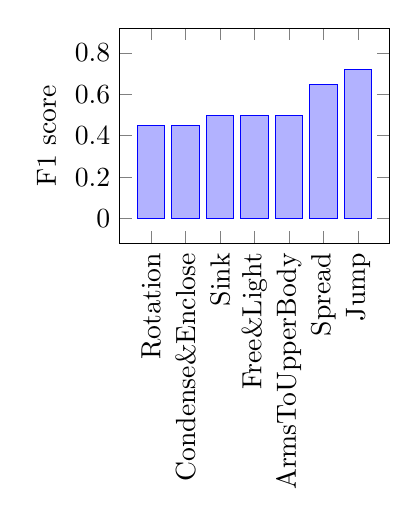
\begin{tikzpicture}
\begin{axis}[
    ymin=0,
    ymax=0.8,
    width=5cm,
    ybar stacked,
    enlargelimits=0.15,
    ylabel={F1 score},
    symbolic x coords={Rotation,Condense\&Enclose,Sink,Free\&Light,ArmsToUpperBody,Spread,Jump},
    xtick=data,
    x tick label style={rotate=90,anchor=east},
    ]
\addplot+[ybar] plot coordinates  {(Rotation,0.45) (Condense\&Enclose,0.45) (Sink,0.5) 
		(Free\&Light,0.5) (ArmsToUpperBody,0.5) (Spread, 0.65) (Jump,0.72)};

\end{axis}
\end{tikzpicture}
\caption{Performance on ordinary  people (non-CMAs) instructed to perform several tasks.}
\label{nonCMAs}
\end{figure}


% An example of a floating figure using the graphicx package.
% Note that \label must occur AFTER (or within) \caption.
% For figures, \caption should occur after the \includegraphics.
% Note that IEEEtran v1.7 and later has special internal code that
% is designed to preserve the operation of \label within \caption
% even when the captionsoff option is in effect. However, because
% of issues like this, it may be the safest practice to put all your
% \label just after \caption rather than within \caption{}.
%
% Reminder: the "draftcls" or "draftclsnofoot", not "draft", class
% option should be used if it is desired that the figures are to be
% displayed while in draft mode.
%
%\begin{figure}[!t]
%\centering
%\includegraphics[width=2.5in]{myfigure}
% where an .eps filename suffix will be assumed under latex, 
% and a .pdf suffix will be assumed for pdflatex; or what has been declared
% via \DeclareGraphicsExtensions.
%\caption{Simulation results for the network.}
%\label{fig_sim}
%\end{figure}

% Note that the IEEE typically puts floats only at the top, even when this
% results in a large percentage of a column being occupied by floats.
% However, the Computer Society has been known to put floats at the bottom.


% An example of a double column floating figure using two subfigures.
% (The subfig.sty package must be loaded for this to work.)
% The subfigure \label commands are set within each subfloat command,
% and the \label for the overall figure must come after \caption.
% \hfil is used as a separator to get equal spacing.
% Watch out that the combined width of all the subfigures on a 
% line do not exceed the text width or a line break will occur.
%
%\begin{figure*}[!t]
%\centering
%\subfloat[Case I]{\includegraphics[width=2.5in]{box}%
%\label{fig_first_case}}
%\hfil
%\subfloat[Case II]{\includegraphics[width=2.5in]{box}%
%\label{fig_second_case}}
%\caption{Simulation results for the network.}
%\label{fig_sim}
%\end{figure*}
%
% Note that often IEEE papers with subfigures do not employ subfigure
% captions (using the optional argument to \subfloat[]), but instead will
% reference/describe all of them (a), (b), etc., within the main caption.
% Be aware that for subfig.sty to generate the (a), (b), etc., subfigure
% labels, the optional argument to \subfloat must be present. If a
% subcaption is not desired, just leave its contents blank,
% e.g., \subfloat[].


% An example of a floating table. Note that, for IEEE style tables, the
% \caption command should come BEFORE the table and, given that table
% captions serve much like titles, are usually capitalized except for words
% such as a, an, and, as, at, but, by, for, in, nor, of, on, or, the, to
% and up, which are usually not capitalized unless they are the first or
% last word of the caption. Table text will default to \footnotesize as
% the IEEE normally uses this smaller font for tables.
% The \label must come after \caption as always.
%
% \begin{table}[!t]
% % increase table row spacing, adjust to taste
% \renewcommand{\arraystretch}{1.3}
% if using array.sty, it might be a good idea to tweak the value of
% \extrarowheight as needed to properly center the text within the cells
% \caption{An Example of a Table}
% \label{table_example}
% \centering
% % Some packages, such as MDW tools, offer better commands for making tables
% % than the plain LaTeX2e tabular which is used here.
% \begin{tabular}{|c||c|}
% \hline
% One & Two\\
% \hline
% Three & Four\\
% \hline
% \end{tabular}
% \end{table}


% Note that the IEEE does not put floats in the very first column
% - or typically anywhere on the first page for that matter. Also,
% in-text middle ("here") positioning is typically not used, but it
% is allowed and encouraged for Computer Society conferences (but
% not Computer Society journals). Most IEEE journals/conferences use
% top floats exclusively. 
% Note that, LaTeX2e, unlike IEEE journals/conferences, places
% footnotes above bottom floats. This can be corrected via the
% \fnbelowfloat command of the stfloats package.



\section{Discussion}
In this study we aimed to develop an automated method for recognizing the motor
characteristics of any human movement captured by the small, inexpensive and
easy to use 3D Kinect camera. We decided to develop the computerized recognition
of movement characteristics based on Laban Movement Analysis (LMA), and chose to
concentrate on recognition of 18 Laban motor elements that were found elsewhere
\cite{shafir2015emotion} as associated with specific emotions. We aimed to develop the
ability to automatically recognize those motor elements from any movement performed by any
person. Although some previous studies have already investigated and
demonstrated automatic recognition of some Laban elements, they often did this
with a much more complex and expensive motion capture system which requires the
moving person to wear special sensors in order to capture his movement (e.g.,
\cite{rett, Aristidou, Chen}).
In addition to their very high price and the need for the moving person to wear
special sensors, such motion capture systems require experts to operate them and
are therefore not practical for commercial use. Those studies that did use
Kinect to capture the movement, and extracted its Laban motor elements, examined
only a few of Laban Efforts (but not other types of Laban motor elements)
\cite{Zacharatos}, or they did it in a limited number of movements performed by
the same person\cite{kim}.
Another line of research that required identification of Laban motor elements
tried to change the bodily emotional expressions of animated characters
\cite{chi2000emote} or of human-like
robots\cite{masuda2009emotion,masuda2010motion}, by modifying some kinematic features of their
movements, which, according to the researchers, represented changes in specific Laban motor elements, that caused the movements to be perceived as expressing different
emotions. However, these studies used a smaller number of Laban motor elements
than examined in our study, and they defined the kinematic features that
represented each motor element based on the meaning of that quality, but without
testing to what extent a movement that incorporates such kinematic feature does
indeed contain the assumed Laban motor element.
\par In order to achieve our aim, we generated video clips of six CMAs moving
various combinations of the 18 Laban motor elements that were examined. The uniqueness
of our study is two folded: first the unique data set that we used as training
set, and second, the methods we used to recognize the Laban motor elements from
these data.
\par The uniqueness of our training data set was that we had a very large
dataset (550 clips), comprised of movements that included specific and known Laban motor
elements, and only those elements. Having movements that were comprised of only
certain motor elements and are not ``contaminated'' by other motor elements,
helped the computer learn more quickly and more accurately which features
characterize each motor element. In addition, by creating the data set with six
professional CMAs we obtained a large variety of movements for each motor
element, all expressing the same motor element. This variety also enhanced the
application of the machine learning techniques to find the best features
characterizing each Laban motor element.
\par In terms of methodology, the main difference between our study and many of
the previous studies was that instead of determining in advance which kinematic
feature(s) represent each Laban element and look only for those features in the
data set in order to recognize that motor element, as was done, for example, by
\cite{aristidou2013motion, kapadia2013efficient,Zacharatos}
, we created thousands of additional different features from the data set, and
activated machine learning algorithms to find which set of features should be
used for recognizing each Laban motor element. Our set of over 6000 features
included some low level features which, similar to the features in
\cite{aristidou2013motion, kapadia2013efficient,Zacharatos} were determined
based on the meaning and assumed kinematic characteristics of the Laban motor element we were trying to capture, but they also included additional
features which were used during the machine learning process.
\par In addition, while some of the previous studies used Bayesian model
\cite{rett, Swaminathan} to capture the features representing each Laban motor
element, we used STL and MTL and found that MTL is superior to STL in recognizing the Laban elements. The
improvement of the average F1 score from a single task learning setting (0.56)
to a multi-task learning setting (0.6) demonstrated the synergy of a shared
model for several correlated tasks.
\par Using machine learning techniques, we succeeded obtaining a recall rate of
38-94\% (65\% on average) and precision rate of 29-100\% (59\% on average) for
the 18 motor elements that were tested. While some of the Laban elements were
relatively easy to learn to automatically recognize, others were more difficult.
The qualities that got higher precision rates were those in which there was a
distinct change in space of either the entire body or parts of it (i.e., a
change in the body's shape): Advance (bringing the chest more forward than the
rest of the body), jump, the combination of going backwards while twisting the
torso, rotation, the combination of rising the torso and bringing the entire
body upward, bringing the arms to touch the upper body, and sinking in the chest
area. Such spatial changes are relatively easy to capture and measure using
kinematics. Indeed several previous studies succeeded, using Baysian models, to
achieve relatively high recognition rates of Laban motor elements that relate to
the space dimension, (67\% in \cite{rett}), or to the body's
shape\cite{Swaminathan}. In contrast to the motor elements that got high
precision rate, there wasn't any obvious characteristic
common to the Laban qualities that were high on recall. Those include some
Efforts: the combination of free and light, and passive weight, a body action:
jump, movements in space: going backwards while twisting the torso, and changes
to the body shape: condensing and enclosing, sinking and spreading. It should be
noted that previous studies found it more difficult to automatically recognize
the Effort qualities of LMA, which are considered to express the person's inner
attitude towards her movement. In our study we succeeded to get a relatively
high F1 score for the combination Efforts of free and light, and for the lack of
Effort weight activation, passive weight, although some of the other Efforts
(e.g., strong, sudden, direct) were still difficult to learn to recognize.
\par Two other achievements of our study were the ability to recognize the Laban
qualities in movements of a CMA using a training set that did not include that
CMA, and the ability to do the same with normative healthy people who did not
have any LMA background and did not intend to produce any specific motor
qualities. The mild degradation of the F1 score from a seen CMA (0.6) to an
unseen (0.57) shows that the generalization ability of the MTL is robust. This
generalization ability probably derived from two unique features of our
methodology. The first is the precision and versatility of our training set as
described above. The other was our focus on the MEN regularization terms, which
kept our model from being too rich, and made it even sparse, and consequently
not over-fitted to the training data.


\section{Conclusion}
In summary, in this study we succeeded with a relatively high success rate to
capture the essence, and develop automatic recognition of 18 LMA motor elements,
using an inexpensive and widely available sensor. We hope that our work will
provide the foundation and inspiration for developing an in-home, inexpensive
LMA based feedback system that will be used for multiple purposes, such as
therapy, arts, video games, communication and human-robot interaction.







% if have a single appendix:
%\appendix[Proof of the Zonklar Equations]
% or
%\appendix  % for no appendix heading
% do not use \section anymore after \appendix, only \section*
% is possibly needed

% use appendices with more than one appendix
% then use \section to start each appendix
% you must declare a \section before using any
% \subsection or using \label (\appendices by itself
% starts a section numbered zero.)
%




% use section* for acknowledgment
\ifCLASSOPTIONcompsoc
  % The Computer Society usually uses the plural form
  \section*{Acknowledgments}
\else
  % regular IEEE prefers the singular form
  \section*{Acknowledgment}
\fi


We would like to thank Ayelet Meltzer, Gahl Liberzon,
Michal Armon, Milca Leon, Sharon Gidron-Peskin and Tara Stepenberg who volunteered
their time and movement to create the data set used in this study.


% Can use something like this to put references on a page
% by themselves when using endfloat and the captionsoff option.
\ifCLASSOPTIONcaptionsoff
  \newpage
\fi



% trigger a \newpage just before the given reference
% number - used to balance the columns on the last page
% adjust value as needed - may need to be readjusted if
% the document is modified later
%\IEEEtriggeratref{8}
% The "triggered" command can be changed if desired:
%\IEEEtriggercmd{\enlargethispage{-5in}}

% references section

% can use a bibliography generated by BibTeX as a .bbl file
% BibTeX documentation can be easily obtained at:
% http://mirror.ctan.org/biblio/bibtex/contrib/doc/
% The IEEEtran BibTeX style support page is at:
% http://www.michaelshell.org/tex/ieeetran/bibtex/
\nocite{bernstein2015laban}
\nocite{ran2015multitask}
\bibliographystyle{IEEEtran}
% argument is your BibTeX string definitions and bibliography database(s)
\bibliography{IEEEabrv,bib}
%
% <OR> manually copy in the resultant .bbl file
% set second argument of \begin to the number of references
% (used to reserve space for the reference number labels box)


% biography section
% 
% If you have an EPS/PDF photo (graphicx package needed) extra braces are
% needed around the contents of the optional argument to biography to prevent
% the LaTeX parser from getting confused when it sees the complicated
% \includegraphics command within an optional argument. (You could create
% your own custom macro containing the \includegraphics command to make things
% simpler here.)
%\begin{IEEEbiography}[{\includegraphics[width=1in,height=1.25in,clip,keepaspectratio]{mshell}}]{Michael Shell}
% or if you just want to reserve a space for a photo:



% You can push biographies down or up by placing
% a \vfill before or after them. The appropriate
% use of \vfill depends on what kind of text is
% on the last page and whether or not the columns
% are being equalized.

%\vfill

% Can be used to pull up biographies so that the bottom of the last one
% is flush with the other column.
%\enlargethispage{-5in}



% that's all folks
\end{document}


